\documentclass [11pt,twoside]{article}
\usepackage[utf8]{inputenc}
\usepackage[T1]{fontenc}

%Page margins, header and footer positions
\usepackage{geometry}
 \geometry{
 a4paper,
 total={210mm,297mm},
 left=25mm,
 right=25mm,
 top=30mm,
 bottom=25mm,
 headsep=7mm}

\interfootnotelinepenalty=10000

%To display filling dots in the TOC for all entries
\usepackage[titles]{tocloft}
\renewcommand{\cftsecleader}{\cftdotfill{\cftdotsep}}

%Define new header and footer style
\usepackage{fancyhdr}

\pagestyle{fancy}
\fancyhf{}
\lhead{\color{Gray}{\small{Travlendar+ project by YOUR NAMES}}}
\lfoot{\textcolor{Gray}{\small{Copyright © 2017, YOUR NAMES – All rights reserved}}}
\rfoot{\textcolor{Gray}{\thepage}}
\renewcommand{\headrulewidth}{0pt}

%PACKAGES
\usepackage{wasysym}
\usepackage{pifont}

\newcommand{\supported}{\ding{52}\xspace}
\newcommand{\unsupported}{\ding{55}\xspace}
\newcommand{\partsupported}{\textcolor{black!40}{\ding{52}}\xspace}
\newcommand{\lowsupported}{\textcolor{black!20}{\ding{52}}\xspace}
\newcommand{\unknowsupported}{\textbf{?}\xspace}

%Font: Times
\usepackage{times}
%Change monospaced font
\renewcommand{\ttdefault}{lmtt}

%tables
\usepackage{tabu}
\usepackage{tabularx}
\usepackage{ltablex}
\usepackage{longtable}
\usepackage{float} % To allow the use of H modifier in long tables

%landscape mode
\usepackage{pdflscape}
\usepackage{rotating}
\usepackage{caption}

%make landscape mode be sensitive to even and odd pages
%start
\def\myrotate{\ifodd\c@page\else-\fi 90}
\makeatletter
\global\let\orig@begin@landscape=\landscape%
\global\let\orig@end@landscape=\endlandscape%
\gdef\@true{1}
\gdef\@false{0}
\gdef\landscape{%
    \global\let\within@landscape=\@true%
    \orig@begin@landscape%
}%
\gdef\endlandscape{%
    \orig@end@landscape%
    \global\let\within@landscape=\@false%
}%
\@ifpackageloaded{pdflscape}{%
    \gdef\pdf@landscape@rotate{\PLS@Rotate}%
}{
    \gdef\pdf@landscape@rotate#1{}%
}
\let\latex@outputpage\@outputpage
\def\@outputpage{
    \ifx\within@landscape\@true%
        \if@twoside%
            \ifodd\c@page%
                \gdef\LS@rot{\setbox\@outputbox\vbox{%
                    \pdf@landscape@rotate{-90}%
                    \hbox{\rotatebox{90}{\hbox{\rotatebox{180}{\box\@outputbox}}}}}%
                }%
            \else%
                \gdef\LS@rot{\setbox\@outputbox\vbox{%
                    \pdf@landscape@rotate{+90}%
                    \hbox{\rotatebox{90}{\hbox{\rotatebox{0}{\box\@outputbox}}}}}%
                }%
            \fi%
        \else%
            \gdef\LS@rot{\setbox\@outputbox\vbox{%
                \pdf@landscape@rotate{+90}%
                \hbox{\rotatebox{90}{\hbox{\rotatebox{0}{\box\@outputbox}}}}}%
            }%
        \fi%
    \fi%
    \latex@outputpage%
}
\makeatother
%end

%graphics
\usepackage{graphicx}
\usepackage[dvipsnames, table]{xcolor}
%If you upload images from PC, you need to insert code for the path here (different for Windows and Unix OS)

%References
%\usepackage{xpatch}
%\usepackage[backend=biber, style=numeric, citestyle=numeric, sorting=none]{biblatex}
%\addbibresource{main.bib}

%Other
\usepackage{ifthen}
\usepackage{xspace}
\usepackage{enumitem}
\usepackage{amssymb}
\usepackage[pdftex, colorlinks]{hyperref}
\newcommand{\comment}[1]{{\color{Red}$\blacktriangleright$ Comment: #1 $\blacktriangleleft$}}


% Some utilities\ldots
\usepackage{soul}
\usepackage{tikz}

\usetikzlibrary{calc}
\usetikzlibrary{decorations.pathmorphing}


\makeatletter

\newcommand{\defhighlighter}[3][]{%
  \tikzset{every highlighter/.style={color=#2, fill opacity=#3, #1}}%
}

\defhighlighter{yellow}{.5}

\newcommand{\highlight@DoHighlight}{
  \fill [ decoration = {random steps, amplitude=1pt, segment length=15pt}
        , outer sep = -15pt, inner sep = 0pt, decorate
       , every highlighter, this highlighter ]
        ($(begin highlight)+(0,8pt)$) rectangle ($(end highlight)+(0,-3pt)$) ;
}

\newcommand{\highlight@BeginHighlight}{
  \coordinate (begin highlight) at (0,0) ;
}

\newcommand{\highlight@EndHighlight}{
  \coordinate (end highlight) at (0,0) ;
}

\newdimen\highlight@previous
\newdimen\highlight@current

\DeclareRobustCommand*\highlight[1][]{%
  \tikzset{this highlighter/.style={#1}}%
  \SOUL@setup
  %
  \def\SOUL@preamble{%
    \begin{tikzpicture}[overlay, remember picture]
      \highlight@BeginHighlight
      \highlight@EndHighlight
    \end{tikzpicture}%
  }%
  %
  \def\SOUL@postamble{%
    \begin{tikzpicture}[overlay, remember picture]
      \highlight@EndHighlight
      \highlight@DoHighlight
    \end{tikzpicture}%
  }%
  %
  \def\SOUL@everyhyphen{%
    \discretionary{%
      \SOUL@setkern\SOUL@hyphkern
      \SOUL@sethyphenchar
      \tikz[overlay, remember picture] \highlight@EndHighlight ;%
    }{%
    }{%
      \SOUL@setkern\SOUL@charkern
    }%
  }%
  %
  \def\SOUL@everyexhyphen##1{%
    \SOUL@setkern\SOUL@hyphkern
    \hbox{##1}%
    \discretionary{%
      \tikz[overlay, remember picture] \highlight@EndHighlight ;%
    }{%
    }{%
      \SOUL@setkern\SOUL@charkern
    }%
  }%
  %
  \def\SOUL@everysyllable{%
    \begin{tikzpicture}[overlay, remember picture]
      \path let \p0 = (begin highlight), \p1 = (0,0) in \pgfextra
        \global\highlight@previous=\y0
        \global\highlight@current =\y1
      \endpgfextra (0,0) ;
      \ifdim\highlight@current < \highlight@previous
        \highlight@DoHighlight
        \highlight@BeginHighlight
      \fi
    \end{tikzpicture}%
    \the\SOUL@syllable
    \tikz[overlay, remember picture] \highlight@EndHighlight ;%
  }%
  \SOUL@
}

\makeatother

% Common abbrev. are set as commands to ensure proper spacing after the dot
\RequirePackage{xspace}
\newcommand{\ie}{i.e.\@\xspace}
\newcommand{\aka}{a.k.a.\@\xspace}
\newcommand{\Ie}{I.e.\@\xspace}
\newcommand{\cf}{cf.\@\xspace}
\newcommand{\Cf}{Cf.\@\xspace}
\newcommand{\eg}{e.g.\@\xspace}
\newcommand{\Eg}{E.g.\@\xspace}
\newcommand{\etal}{et al.\@\xspace}
\newcommand{\etc}{etc.\@\xspace}
\newcommand{\wrt}{w.r.t.\@\xspace}
\newcommand{\Wrt}{W.r.t.\@\xspace}



\date{}

\DeclareUnicodeCharacter{202F}{AAAAAA}
\begin{document}
\fontfamily{ppl}\selectfont

%TITLE PAGE
\setlength\parindent{18pt}
\begin{titlepage}


%LOGO

{\begin{table}[t!]
\centering
\begin{tabu} to \textwidth { X[1.3,r,p] X[1.7,l,p] }
\textcolor{Blue}
{\textbf{\small{Software Engineering 2\break CLup project by\break Robert Medvedec\break Toma Sikora}}} & 
\includegraphics[scale=0.5]{Images/PolimiLogo}
\end{tabu}
\end{table}}~\\ [7cm]

%TITLE 

\begin{flushleft}

%Replace the text string with your title
{\textcolor{Blue}{\textbf{\Huge{Implementation  and  Test  deliverable}}}} \\ [1cm]

\end{flushleft}

\end{titlepage}

%Define deliverable specific info
%Replace cell contents where needed
\begin{table}[h!]
\begin{tabu} to \textwidth { X[0.3,r,p] X[0.7,l,p] }
\hline

\break\textbf{Deliverable:} & \break ITD\\
\break\textbf{Title:} & \break  Implementation  and  Test  deliverable \\
\textbf{Authors:} & Robet Medvedec, Toma Sikora \\
\textbf{Version:} & 1.0 \\ 
\textbf{Date:} & 7-February-2021 \\
\textbf{Download page:} & \url{https://github.com/robertodavinci/Software_Engineering_2_Project_Medvedec_Sikora/Implementation/Clup} \\
\break\textbf{Copyright:} & \break Copyright © 2021, R. Medvedec, T. Sikora – All rights reserved\break\\
\hline
\end{tabu}
\end{table}




\setcounter{page}{2}


%------------------------------------------------------------------------------------------------------------------------------------------------
\newpage
\addcontentsline{toc}{section}{Table of Contents}
\tableofcontents
\newpage
\addcontentsline{toc}{section}{List of Figures}
\listoffigures
\addcontentsline{toc}{section}{List of Tables}
\listoftables

%------------------------------------------------------------------------------------------------------------------------------------------------
\clearpage
{\color{Blue}{\section{Introduction}}}
\label{sect:introduction}
\subsection{Purpose}
\hspace{\parindent}This document provides a detailed view of the architecture and the implementation of the CLup system. Based on both RASD and DD documents provided in this project, that can both be found on the above provided GitHub page, this document specifies the development process and used frameworks and philosophies, as well as explains the code structure and design rationale behind the whole system.

The system implementation is done as an Android app that is available for every Android device that supports Android 8.0 and above. 

Detailed code can be found on provided GitHub page and it can also be imported as an Android Studio project in order to make adjustments to the app.


\newpage

\subsection{Scope}
\hspace{\parindent}CLup is a simple application that helps store managers with handling large crowds inside their store and store customers with planning more efficient and safe grocery shops. The target audience for this application includes every person that shops for groceries in a store, which includes almost all demographics fall into this category. 

Faced with a worldwide pandemic of the COVID-19 virus countries across the world imposed strict health measures in line with the recommendations of the WHO. To combat the spread of the virus, governments introduced decrees that limited the movement of the population to a certain degree. Only essential movement, such as: going to work, grocery shopping or outdoor exercise, was deemed acceptable. Although successful in the mitigation of the disease, the act put a serious strain on society on many levels. To help reduce the stress and anxiety, many aspects of everyday life involving close contact can be considered and improved upon. 

This project aims to help with, and resolve the issues surrounding grocery shopping. As we all know, grocery shopping is an essential activity which involves close contact inside the store. Since the COVID-19 virus spreads mainly through airborne particles, this activity plays a key role in its mitigation. To reduce crowding inside the stores, supermarkets need to restrict access to their store and keep the number of people inside below the optimal maximum capacity. 

The main idea is to enable store customers to enter a queue from home (or wherever they find themselves) through simple interaction with the application. 

\newpage

\subsection{Definitions, Acronyms, Abbreviations}
\subsubsection{Definitions}
\begin{itemize} 
	\item \textbf{Application}: a computer (mobile) program that is designed for a particular purpose. 
	\item \textbf{QR code}: a machine-readable code consisting of an array of black and white squares, typically used for storing URLs or other information for reading by the camera or a scanner. 
	\item \textbf{Smartphone}: a mobile phone that performs many of the functions of a computer, typically having a touchscreen interface, internet access, and an operating system capable of running downloaded apps. 
	\item \textbf{Google Maps}: a web mapping service developed by Google, used both as a standalone app and as an integrated mapping solution in most of the apps.
	\item \textbf{Android}: most popular operating system for smartphones and tablets, developed by Google and partners.
\end{itemize}
\subsubsection{Acronyms}
\begin{itemize}
	\item \textbf{RASD}: Requirement Analysis and Specification Document
	\item \textbf{COVID-19}: Virus responsible for the spread of the coronavirus disease 2019
	\item \textbf{CLup}: Customer Line-up
	\item \textbf{API}: Application programming interface, computing interface which defines interactions between multiple software intermediaries 
	\item \textbf{WHO}: World Health Organization
	\item \textbf{GUI}: Graphical user interface
	\item \textbf{DB}: Database
	\item \textbf{REST}: Representational state transfer - software architectural style used in web services
	\item \textbf{AES}: Advanced Encryption Standard
\end{itemize}
\subsubsection{Abbreviations}
\begin{itemize}
	\item \textbf{Gn}: nth goal.
	\item \textbf{Rn}: nth functional requirement.
	\item \textbf{App}: Application.
\end{itemize}

\newpage
\subsection{Revision History}
\begin{itemize}
	\item \textbf{Version 1.0}: First .tex document created and added all together; 7th February 2021
\end{itemize}

\newpage
\subsection{Reference Documents}
\begin{itemize}
	\item Specification document "R\&DD Assignment A.Y. 2020-2021.pdf"
	\item Specification document "Implementation Assignment A.Y. 2020-2021.pdf"
	\item Presentations Software Engineering 2, Politecnico di Milano
	\item Star UML - Program used for creating diagrams
	\item Fundementals of Software Engineering - C. Ghezzi, M. Jazayeri, D. Mandrioli
\end{itemize}


\newpage
\subsection{Document Structure}
\hspace{\parindent} WRITE SOMETHING SMART AT THE END HERE


%------------------------------------------------------------------------------------------------------------------------------------------------
\clearpage
{\color{Blue}{\section{Requirements}}}
\label{sect:requirements}
To further clarify and reason the implementation components proposed in the \textbf{\hyperref[fig:componentdiagram1]{main component diagram}} this chapter connects them with the goals and requirements, specified in the RASD document. Each goal \textbf{[Gn]} will be presented, and connected with the mapped requirements \textbf{[Rn]} and responsible design counterparts.\newline


\begin{table}[H]
\begin{flushleft}
\begin{tabular}{|l|l|}
\hline
R1&The user must be able to select a specific store in which they want \\ & to do the shopping.\\
\hline
R2&The user must be able to request a number and a ticket.\\
\hline
R3&The user must be able to receive a number and a ticket. \\
\hline
R4&The user must be able to physically retrieve a ticket from the printer \\   &  containing a number and a QR code.\\
\hline
R5&A new ticket must be printed whenever a user physically retrieves the old one.\\
\hline
R6&The store manager must be able to scan a QR code.\\
\hline
R7&The store manager must be informed by the application if a user tries to enter the \\ & store out of order.\\
\hline
R8&The store manager must be informed when the capacity of the store is full.\\
\hline
R9&The store manager must be able to alert the system whenever a customer \\ & exits the store.\\
\hline
R10&The store manager must be provided with the login credentials upon \\ & request to the system administrator.\\
\hline
R11&Allow the user to receive a precise estimation of waiting time when \\ &  retrieving a number.\\
\hline
R12&The system must calculate an estimation of the waiting time based on data.\\
\hline
R13&The system must be able to update its estimated waiting time in real time.\\
\hline
R14&The system must be able to send an update to the user in specific \\ & intervals regarding estimated waiting time until it's their turn.\\
\hline
R15&The user must be able to request to see all the available timeslots  in that \\ & specific store.\\
\hline
R16&The system must be able to provide the user with the list of all available timeslots \\ & upon the request.\\
\hline
R17&The user must be able to select a specific timeslot.\\
\hline
R18&The user must be able to receive a confirmation of his timeslot reservation, along \\ & with a number and a ticket.\\
\hline
R19&Allow the user to be at most five minutes late for his reservation before cancelling \\ &  his ticket.\\
\hline
R20&The user must be able to specify expected duration of his visit to the store.\\
\hline
\end{tabular}
\end{flushleft}
\caption{\textbf{Requirements table}}
\label{tab:reqtable}
\end{table}

\newpage
\begin{table}
\begin{flushleft}
\begin{tabular}{|l|l|}
\hline
\cellcolor[HTML]{EC8D78}& \cellcolor[HTML]{F4D5CE}Allow the user to retrieve a number through the application.\\
\cline{2-2}
\cellcolor[HTML]{EC8D78}& \cellcolor[HTML]{F4D5CE}Requirements: R1, R2, R3\\
\cline{2-2}
\cellcolor[HTML]{EC8D78}&Components:\\

\cellcolor[HTML]{EC8D78}G1.1&\quad\quad AndroidApp/IPhoneApp\\

\cellcolor[HTML]{EC8D78}&\quad\quad	Director \\

\cellcolor[HTML]{EC8D78}&\quad\quad	StoreSelectionManager \\

\cellcolor[HTML]{EC8D78}&\quad\quad	RequestManager \\

\cellcolor[HTML]{EC8D78}&\quad\quad\quad\quad	TicketService \\

\cellcolor[HTML]{EC8D78}&\quad\quad\quad\quad	QueueService \\

\cellcolor[HTML]{EC8D78}&\quad\quad\quad\quad	ScheduleService\\ 

\cellcolor[HTML]{EC8D78}&\quad\quad	DBService and DB \\
\hline
\end{tabular}
\end{flushleft}
\caption{\textbf{Components table - Goal 1.1}}
\label{tab:comp1}
\end{table}


\begin{table}
\begin{flushleft}
\begin{tabular}{|l|l|}
\hline
\cellcolor[HTML]{EC8D78}& \cellcolor[HTML]{F4D5CE}Allow the user to retrieve a number physically from the printer.\\
\cline{2-2}
\cellcolor[HTML]{EC8D78}& \cellcolor[HTML]{F4D5CE}Requirements: R4, R5 \\
\cline{2-2}
\cellcolor[HTML]{EC8D78}&Components:\\

\cellcolor[HTML]{EC8D78}G1.2&\quad\quad	Director \\

\cellcolor[HTML]{EC8D78}&\quad\quad	StoreSelectionManager \\

\cellcolor[HTML]{EC8D78}&\quad\quad	RequestManager \\

\cellcolor[HTML]{EC8D78}&\quad\quad\quad\quad	TicketService \\

\cellcolor[HTML]{EC8D78}&\quad\quad\quad\quad	QueueService \\

\cellcolor[HTML]{EC8D78}&\quad\quad\quad\quad	ScheduleService\\ 

\cellcolor[HTML]{EC8D78}&\quad\quad	DBService and DB \\
\hline
\end{tabular}
\end{flushleft}
\caption{\textbf{Components table - Goal 1.2}}
\label{tab:comp1}
\end{table}

\begin{table}
\begin{flushleft}
\begin{tabular}{|l|l|}
\hline
\cellcolor[HTML]{EC8D78}& \cellcolor[HTML]{F4D5CE}Allow the store manager to control the entrance of customers via QR code scanning.\\
\cline{2-2}
\cellcolor[HTML]{EC8D78}& \cellcolor[HTML]{F4D5CE}Requirements: R6, R7, R8, R9, R10\\
\cline{2-2}
\cellcolor[HTML]{EC8D78}&Components:\\

\cellcolor[HTML]{EC8D78}G2&\quad\quad AndroidApp/IPhoneApp\\

\cellcolor[HTML]{EC8D78}&\quad\quad	Director \\

\cellcolor[HTML]{EC8D78}&\quad\quad	LoginManager \\

\cellcolor[HTML]{EC8D78}&\quad\quad	StoreSelectionManager \\

\cellcolor[HTML]{EC8D78}&\quad\quad	StoreManager \\

\cellcolor[HTML]{EC8D78}&\quad\quad\quad\quad EnterService \\

\cellcolor[HTML]{EC8D78}&\quad\quad\quad\quad ExitService \\

\cellcolor[HTML]{EC8D78}&\quad\quad	RequestManager \\

\cellcolor[HTML]{EC8D78}&\quad\quad	DBService and DB \\
\hline
\end{tabular}
\end{flushleft}
\caption{\textbf{Components table - Goal 2}}
\label{tab:comp1}
\end{table}


\newpage

\begin{table}
\begin{flushleft}
\begin{tabular}{|l|l|}
\hline
\cellcolor[HTML]{EC8D78}& \cellcolor[HTML]{F4D5CE}Allow the user to receive precise calculations of the waiting time.\\
\cline{2-2}
\cellcolor[HTML]{EC8D78}& \cellcolor[HTML]{F4D5CE}Requirements: R11, R12\\
\cline{2-2}
\cellcolor[HTML]{EC8D78}&Components:\\

\cellcolor[HTML]{EC8D78}G3&\quad\quad AndroidApp/IPhoneApp\\

\cellcolor[HTML]{EC8D78}&\quad\quad	Director \\

\cellcolor[HTML]{EC8D78}&\quad\quad	RequestManager \\

\cellcolor[HTML]{EC8D78}&\quad\quad\quad\quad	DistanceService \\

\cellcolor[HTML]{EC8D78}&\quad\quad	GoogleMapsService\\ 

\cellcolor[HTML]{EC8D78}&\quad\quad	DBService and DB \\
\hline
\end{tabular}
\end{flushleft}
\caption{\textbf{Components table - Goal 3}}
\label{tab:comp1}
\end{table}



\begin{table}
\begin{flushleft}
\begin{tabular}{|l|l|}
\hline
\cellcolor[HTML]{EC8D78}& \cellcolor[HTML]{F4D5CE}Allow the user to be updated on the store waiting time situation.\\
\cline{2-2}
\cellcolor[HTML]{EC8D78}& \cellcolor[HTML]{F4D5CE}Requirements: R13, R14\\
\cline{2-2}
\cellcolor[HTML]{EC8D78}&Components:\\

\cellcolor[HTML]{EC8D78}G4&\quad\quad AndroidApp/IPhoneApp\\

\cellcolor[HTML]{EC8D78}&\quad\quad	Director \\

\cellcolor[HTML]{EC8D78}&\quad\quad	RequestManager \\

\cellcolor[HTML]{EC8D78}&\quad\quad	GoogleMapsService \\

\cellcolor[HTML]{EC8D78}&\quad\quad	DBService and DB \\
\hline
\end{tabular}
\end{flushleft}
\caption{\textbf{Components table - Goal 4}}
\label{tab:comp1}
\end{table}




\begin{table}
\begin{flushleft}
\begin{tabular}{|l|l|}
\hline
\cellcolor[HTML]{EC8D78}& \cellcolor[HTML]{F4D5CE}Allow the user to "book a visit" to the store.\\
\cline{2-2}
\cellcolor[HTML]{EC8D78}& \cellcolor[HTML]{F4D5CE}Requirements: R15, R16, R17, R18, R19, R20\\
\cline{2-2}
\cellcolor[HTML]{EC8D78}&Components:\\

\cellcolor[HTML]{EC8D78}G5&\quad\quad AndroidApp/IPhoneApp\\

\cellcolor[HTML]{EC8D78}&\quad\quad	Director \\

\cellcolor[HTML]{EC8D78}&\quad\quad	StoreSelectionManager \\

\cellcolor[HTML]{EC8D78}&\quad\quad	RequestManager \\

\cellcolor[HTML]{EC8D78}&\quad\quad\quad\quad	BookAVisitService \\

\cellcolor[HTML]{EC8D78}&\quad\quad\quad\quad	TicketService \\

\cellcolor[HTML]{EC8D78}&\quad\quad\quad\quad	QueueService\\ 

\cellcolor[HTML]{EC8D78}&\quad\quad\quad\quad	ScheduleService\\ 

\cellcolor[HTML]{EC8D78}&\quad\quad	DBService and DB \\
\hline
\end{tabular}
\end{flushleft}
\caption{\textbf{Components table - Goal 5}}
\label{tab:comp1}
\end{table}



%------------------------------------------------------------------------------------------------------------------------------------------------
\clearpage
{\color{Blue}{\section{Adopted Development Frameworks}}}
\label{sect:adopteddevelopmentframeworks}
\subsection{Adopted programming languages and frameworks}
\hspace{\parindent} The CLup app as already mentioned has been developed in Android Studio, an IDE for building Android apps based on IntelliJ IDEA software from JetBrains. Android Studio can be used with three programming languages - Kotlin, Java, and C++ , all used for object oriented programming of the app. \newline
Our choice was to go with Java since that's the language we're most familiar with and a language that exists a lot longer than Kotlin, which is Google's preferred language for Android app dev, so more examples can be found online for easier referencing. \newline
Java also offers vast and detailed documentation as well as similar syntax to some other more popular languages, contrary to Kotlin. \newline
Android Studio also uses an internal UI design tool, which is based on XML language that uses layouts, items, and resources for designing and creating different app screens. It features a real-time design screen making an UI design a lot smoother and faster experience. \newline
During the development we have used a Google Pixel 3 virtual machine, that is also integrated in Android Studio, for testing and other app-related purposes.\newline 
Several phones of different sizes, vendors, and Android versions have been used for real-life testing, and those are: Samsung Galaxy Note 9, Xiaomi Redmi Note 9 Pro, and Huaweii P Smart.  \newline
Even though our original plan was to use MySQL database for the backend of this project, we have decided to use Google's Firebase that was mentioned as an alternative in the Design document. More details on this design choice in the sections below.

\subsection{Adopted additional algorithms and middleware}
\hspace{\parindent} One of the APIs that was planned to be used, Google Maps API, did not make the cut in this version. The reasoning behind that is already explained in the previous chapter and it touches on the lack of "Book a visit" feature that was not required to be made for smaller groups. Using this API would further complicate things and we did not find it necessary just for the ticket queueing function of the app, since this function would mostly be used on the fly and without too much planning, which would mean that the customers would already know to which store they are going and how to get there. \newline

One of the main challenges of the system was securing a proper encryption for the QR code which is to be scanned by the store manager. If we put no encryption on it, the customers can easily scan the code on their own, see how it looks, and the create their own QR codes to skip lines and get faster access to the store. \newline
For that reason we have decided to use AES or Advanced Encryption Standard which is a specification for electronic data encryption. It is one of the most widely used standards in the world and regarded as one of the most secure. \newline

This standard uses either 128, 192, or 256 bit keys to encode and decode data. It is also symmetrical, making it easier to do encryption/decryption without exchanging keys. \newline

The way AES works is that it takes plaintext and a key, encodes it using a special algorithm, and then sends the ciphertext to the destination. The receiver receiver the ciphertext and decodes it using the same key, getting the original message. \newline

\begin{figure}[H]
\centering
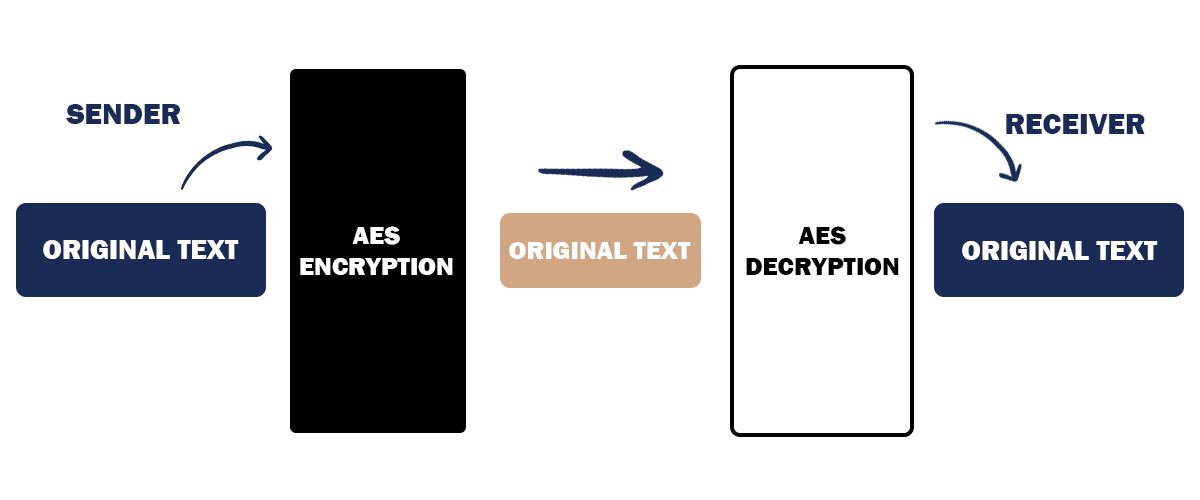
\includegraphics[width=\textwidth]{Images/AES}
\caption{\label{fig:aes}\textbf{AES sketch}}
\end{figure}

Each store in our database has a unique 128 bit key with mixed characters. This key is used for encryption when requesting a ticket and then for decryption when scanning a ticket. The key is not sent at any moment over the network and it's not shown to the customer or the store manager at any time, making the app very secure in that regard.\newline
If user tries to scan the QR code, they will get something like this:\newline

"-112w-22w34w-41w34w-120w2w-22w87w-93w-41w65w11".\newline

Good luck with trying to get any data from that! Even NSA uses it.
Our encryption code generates random signed 8 bit integers which are then interleaved with a letter, "w" in this scenario, for easier decryption later. The code for the algorithm is provided here.\newline

\textbf{Entities - StrongAES}

\begin{lstlisting}
// StrongAES.java
package com.example.clup;

import java.security.Key;
import javax.crypto.Cipher;
import javax.crypto.spec.SecretKeySpec;
public class StrongAES
{
    // function that Encrypts and Decrypts data
    public byte[] AESEncrypt(String plaintext, String key){
        try {
            Key aesKey = new SecretKeySpec(key.getBytes(), "AES");
            Cipher cipher = Cipher.getInstance("AES");
            // encrypt the text
            cipher.init(Cipher.ENCRYPT_MODE, aesKey); // encrypted with a key
            byte[] cy = cipher.doFinal(plaintext.getBytes()); // encryption is returned in bytes[] array
            //System.out.println(cy);
            return cy;
        }
        catch(Exception e){
            //return 'D';
            return "false".getBytes();
        }
    }

    public String AESDecrypt(byte[] cyphertext, String key){
        try {
            Key aesKey = new SecretKeySpec(key.getBytes(), "AES");
            Cipher cipher = Cipher.getInstance("AES");
            cipher.init(Cipher.DECRYPT_MODE, aesKey); // decrypted with a key
            String cy2 = new String(cipher.doFinal(cyphertext)); // decryption is returned in String
            //System.out.println(cy2);
            return cy2;
        }
        catch(Exception e){
            System.err.println(e);
            return "Error";
        }
    }
   }
\end{lstlisting}


\subsection{Database model}
\hspace{\parindent} Google's Firebase is a very powerful databse tool for two reason - it is very simple and it's easily integrated with Android apps. It is not a standard database tool that uses SQL language (it is NoSQL), but rather separates its data by using JSON structures and a classic key-value methodology. Every item can have a key and a value, as well as be a parent and have multiple children. However, any item that has a child or children cannot have any values, but is rather just represented with a key. \newline

This all makes extracting data very simple, but it generates a problem with data multiplication since there is no way of connecting some items with a pointer or by id. What must be done is a manual data copying, which increases size and complexity of the structure. \newline

Android Studio and the whole Android environment has already built in functions that make working with Firebase much easier, which was the main reason for this selection. Functions for user registration and login are already set up and are super secure, not even requiring storing user password in the database. \newline

The whole Firebase interface is also very well done and allows maximum customization as well as adaptability to the certain project. It is located on a Google server, so there is no need to worry about any other sever that runs a normal database, since Google servers are always up and have very small limitations, at least for a smaller scale project. \newline

You can see the way we have structured our database in the following examples. 

\begin{figure}[H]
\centering
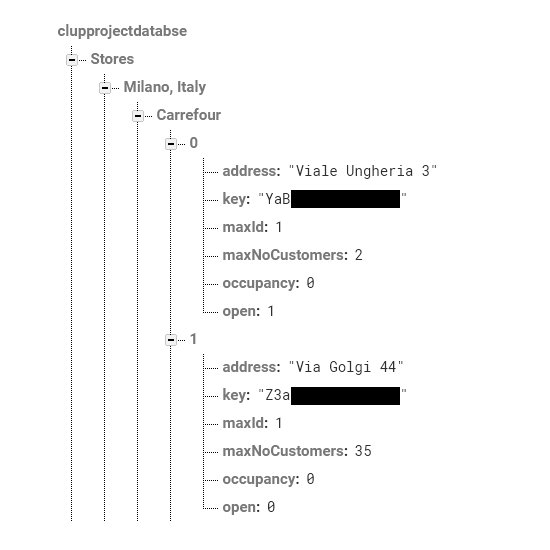
\includegraphics[width=\textwidth]{Images/Firebase1}
\caption{\label{fig:fire1}\textbf{Our Firebase database 1}}
\end{figure}
\begin{figure}[H]
\centering
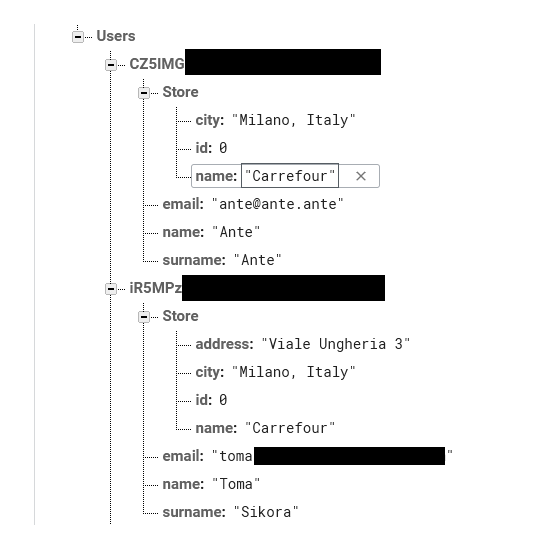
\includegraphics[width=\textwidth]{Images/Firebase2}
\caption{\label{fig:fire2}\textbf{Our Firebase database 2}}
\end{figure}


The two main items are "Stores" and "Users". Stores are ordered by cities, then by store names, and finally by id. Each store has an address, a key, a current ticket id, a maximum number of customers, an occupancy number, and an open indicator. Also, each store has another set of children "Tickets", which is created dynamically. \newline

Each user is defined by "UserID" which is a Firebase identification. Connected to the user are a specific Store, which here only consists of a city, an ID, and a name, so we can reference it in the other "Store" structure, as well as an email, a name, and a surname, with the latter two being used only for registration, which has been omitted from the final app version. Therefore store managers and stores are added manually for additional security and data consistency. \newline

The main Firebase issue is the data retrieval - sometimes the servers take up to 5 seconds to return simple data! In this case it is not a major issue, since the speed is not the most important function of the application, but the server dependability of getting the data back on time can cause some problems. \newline

All in all, in case of a a real-world app for a much larger scale, we would probably transfer to MySQL mainly because of speed and stability which are not strong sides of Firebase. \newline

%------------------------------------------------------------------------------------------------------------------------------------------------
\clearpage
{\color{Blue}{\section{Code Structure}}}
\label{sect:codestructure}
\subsection{Classes, Interfaces, and Enumerations}
\hspace{\parindent}
\subsection{Code examples}

%------------------------------------------------------------------------------------------------------------------------------------------------
\clearpage
{\color{Blue}{\section{Testing}}}
\label{sect:testing}
\subsection{Implemented requirements}
\hspace{\parindent} The list of requirements and their implementation status is included in ITD file. Testing has been done on these implementations and the comments on whether they are correctly implemented or not are next to the requirement name in the following list:

\begin{itemize}
\item[\textbf{R.1}]\textbf{ The system shall allow customers to line-up remotely in a store queue.}\newline \textbf{Implementation status}: Implemented\newline \textbf{Comments}: The line-up implementation doesn't really exist, queueing is not managed by the time the ticket has been requested or the ticket number, but rather every ticket scan is accepted, making the store employee in charge for the decision on who can enter the store and not the system. The virtual line-up exists, but it's not ordered in any way, making the whole point of the line-up non existent.
\item[\textbf{R.2}] \textbf{The system shall generate a new ticket when a customer enters a queue}\newline \textbf{Implementation status}: Implemented\newline \textbf{Comments}: Implementation tested and working correctly.
\item[\textbf{R.3}]\textbf{The system shall allow customers which do not have a smartphone to get a ticket in place.}\newline \textbf{Implementation status}: Not implemented\newline \textbf{Comments}: /
\item[\textbf{R.4}]\textbf{The system shall allow customers to view the number of people lined up in a queue}\newline \textbf{Implementation status}: Implemented\newline \textbf{Comments}: Implementation tested and working correctly.
\item[\textbf{R.5}]\textbf{The system shall give customers an estimated waiting time.}\newline \textbf{Implementation status}:Partially implemented\newline \textbf{Comments}: Time estimation is equal to 1 person per 15 minutes. The estimation doesn't really work correctly since there is no store queueing and no way or determining how many people are in front, making estimation always be either 0 or 15 minutes.
\item[\textbf{R.6}]\textbf{The system shall fetch the GPS position while the user has retrieved a store pass.}\newline \textbf{Implementation status}:Not implemented\newline \textbf{Comments}: /
\item[\textbf{R.7}]\textbf{The system shall allow customers to leave a queue.}\newline \textbf{Implementation status}:Implemented\newline \textbf{Comments}: Customer can delete the ticket anytime, therefore leaving the queue. Implementation tested and working correctly.
\item[\textbf{R.8}]\textbf{The system shall allow customers to filter stores by name.}\newline \textbf{Implementation status}:Implemented\newline \textbf{Comments}: Implementation tested and working correctly.
\item[\textbf{R.9}]\textbf{The system shall notify customers when it’s time to leave for the store.}\newline \textbf{Implementation status}:Not implemented\newline \textbf{Comments}: /
\item[\textbf{R.10}]\textbf{The system shall allow customers to book-a-visit to the store and send them the confir-mation link and receipt via email.}\newline \textbf{Implementation status}:Not implemented\newline \textbf{Comments}: /
\item[\textbf{R.11}]\textbf{The system shall allow book-a-visit customers to specify the main categories of itemthey intend to buy.}\newline \textbf{Implementation status}:Not implemented\newline \textbf{Comments}: /
\item[\textbf{R.12}]\textbf{The system shall allow customers to delete a store pass.}\newline \textbf{Implementation status}:Partially implemented \newline \textbf{Comments}: There are no bookings because "Book a visit" feature doesn't exist. Ticket deletion working correctly.
\item[\textbf{R.13}]\textbf{The system shall notify customers when a ticket or booked visit is deleted.}\newline \textbf{Implementation status}:Not implemented\newline \textbf{Comments}: /
\item[\textbf{R.14}]\textbf{The system shall accept bookings based onto the already booked category items.}\newline \textbf{Implementation status}:Not implemented\newline \textbf{Comments}: /
\item[\textbf{R.15}]\textbf{The system shall allow a registered store manager to login by using their credentials.}\newline \textbf{Implementation status}:Implemented\newline \textbf{Comments}: Implementation tested and working correctly.
\item[\textbf{R.16}]\textbf{The system shall allow store managers to view the current status of people inside the store.}\newline \textbf{Implementation status}:Implemented\newline \textbf{Comments}: Implementation tested and working correctly.
\item[\textbf{R.17}]\textbf{The system shall allow store managers to view the current status of people in the queue.}\newline \textbf{Implementation status}:Implemented\newline \textbf{Comments}: Implementation tested and working correctly.
\item[\textbf{R.18}]\textbf{The system shall allow store managers to view the booked visits to the store.}\newline \textbf{Implementation status}:Not implemented\newline \textbf{Comments}: /
\item[\textbf{R.19}]\textbf{The system shall allow store managers to set a maximum cap of people inside the store.}\newline \textbf{Implementation status}:Implemented\newline \textbf{Comments}: Implementation tested and working correctly.
\item[\textbf{R.20}]\textbf{The system shall allow store managers to delete tickets and booked visits.}\newline \textbf{Implementation status}:Partially implemented \newline \textbf{Comments}: There are no bookings because "Book a visit" feature doesn't exist. Ticket deletion working correctly.
\item[\textbf{R.21}]\textbf{The system shall allow a registered store employee to login by using their credentials.}\newline \textbf{Implementation status}:Implemented \newline \textbf{Comments}: Implementation tested and working correctly.
\item[\textbf{R.22}]\textbf{The system shall allow store employee to view the current status of people inside the store.}\newline \textbf{Implementation status}:Implemented \newline \textbf{Comments}: Implementation tested and working correctly.
\item[\textbf{R.23}]\textbf{The system shall allow store employee to view the current status of people in the queue.}\newline \textbf{Implementation status}:Implemented \newline \textbf{Comments}: Implementation tested and working correctly.
\item[\textbf{R.24}]\textbf{The system shall allow store employee to scan QR codes.}\newline \textbf{Implementation status}:Implemented \newline \textbf{Comments}: Implementation tested and working correctly.
\item[\textbf{R.25}]\textbf{The system shall allow store employee to validate store passes.}\newline \textbf{Implementation status}:Partially implemented \newline \textbf{Comments}: there are no bookings because "Book a visit" feature doesn't exist. Ticket scanning working correctly.
\item[\textbf{R.26}]\textbf{The system shall allow CLup admins to register new supermarkets.}\newline \textbf{Implementation status}:Implemented \newline \textbf{Comments}: Implementation tested and working correctly. New supermarkets can be registered with name, full address, image, and work hours. No two stores of the same name and faulty work hours can be registered.
\item[\textbf{R.27}]\textbf{The system shall generate new manager and staff credentials for each supermarket registered.}\newline \textbf{Implementation status}:Implemented \newline \textbf{Comments}: Implementation tested and working correctly.
\end{itemize}

We have also replicated (manually) all the Unit and System tests defined in ITD1.0.pdf file under chapters 5.1 and 5.3. We have gotten the same results as the creators of the system. Here are a couple of examples and error messages received when trying different "bad" actions.

\begin{figure}[!htb]
\centering
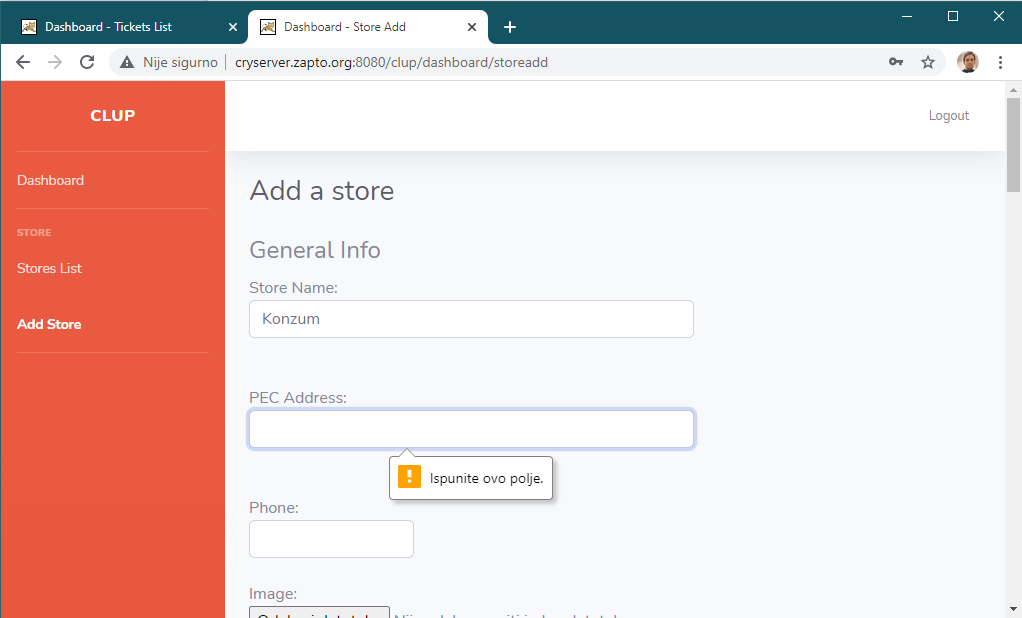
\includegraphics[width=\textwidth]{Images/FieldEmpty}
\captionsetup{justification=centering}
\caption{\label{fig:desktoperr1}\textbf{Left empty field when creating a store}}
\end{figure}
\begin{figure}[!htb]
\centering
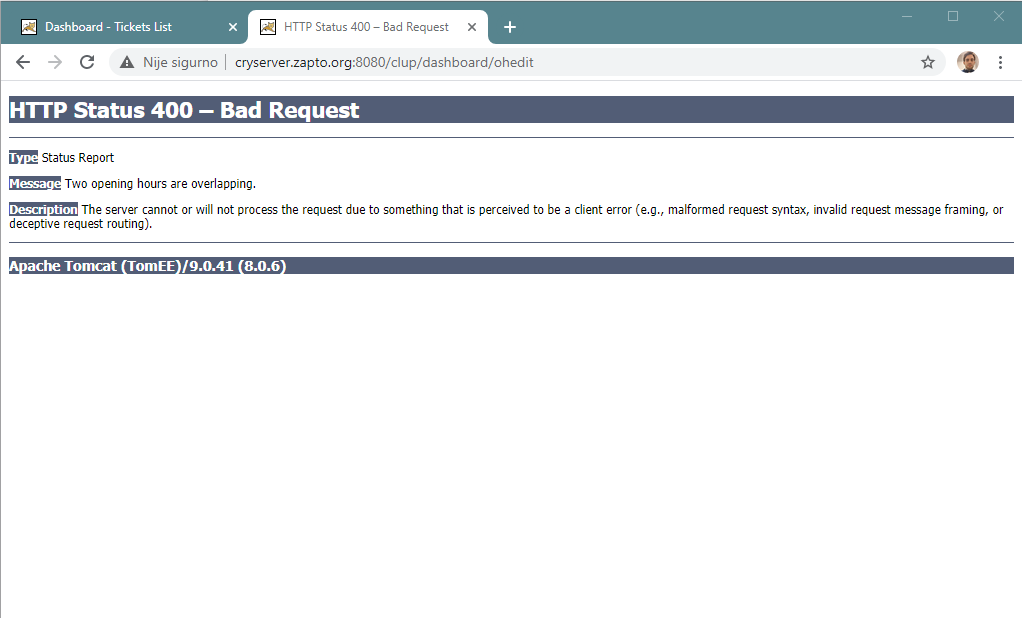
\includegraphics[width=\textwidth]{Images/BadHours}
\captionsetup{justification=centering}
\caption{\label{fig:desktoperr2}\textbf{Bad work hours written - two overlapping intervals}}
\end{figure}
\begin{figure}[!htb]
\centering
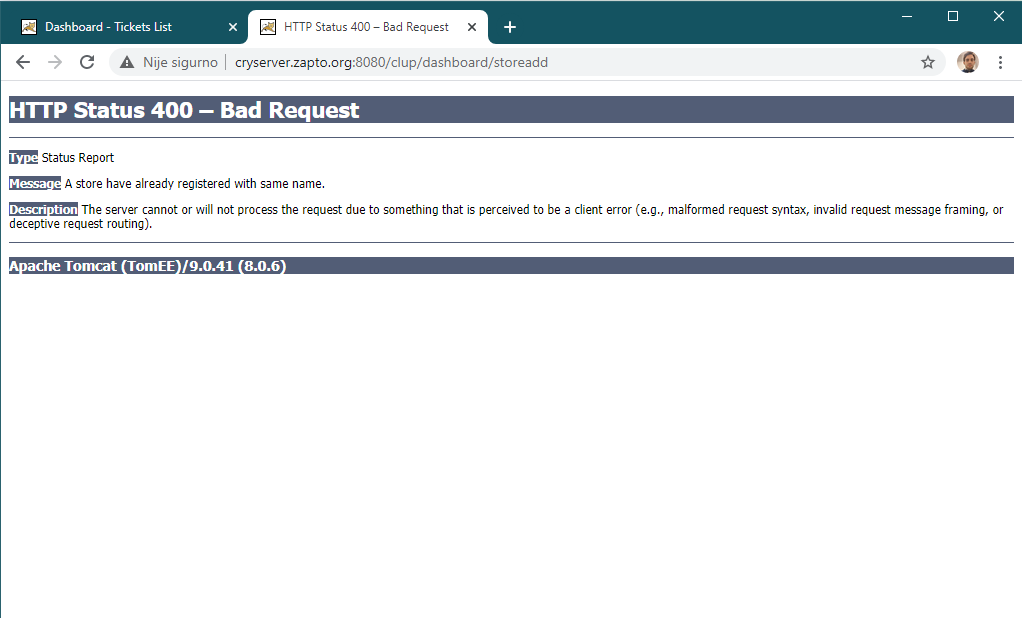
\includegraphics[width=\textwidth]{Images/SameName}
\captionsetup{justification=centering}
\caption{\label{fig:desktoperr3}\textbf{Two stores of the same name error}}
\end{figure}

\begin{figure}[!htb]
\centering
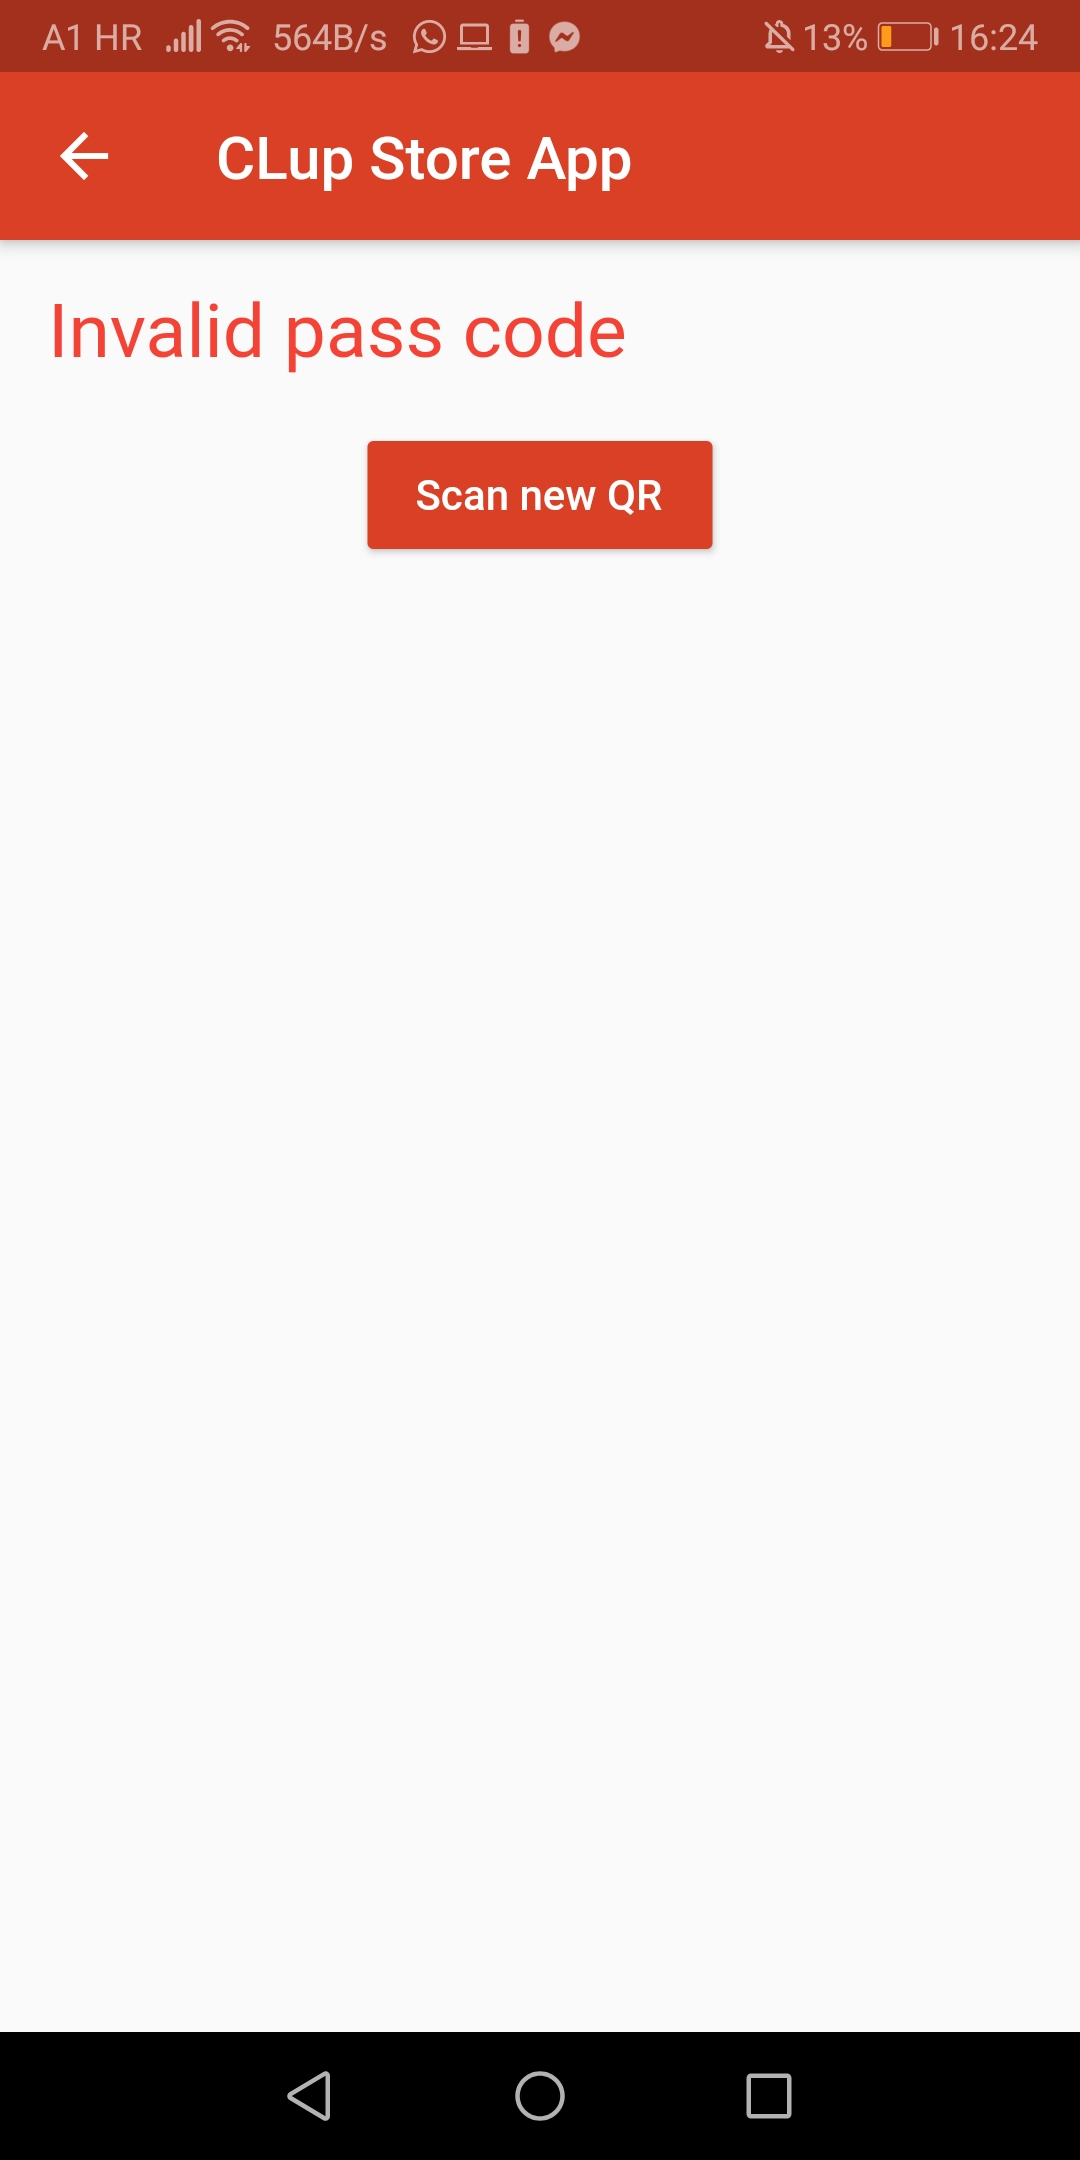
\includegraphics[width=0.35\textwidth]{Images/InvalidScan}
\captionsetup{justification=centering}
\caption{\label{fig:appandroiderr3}\textbf{Invalid QR code scan error}}
\end{figure}

\begin{figure}[!htb]
\centering
\begin{minipage}{0.45\textwidth}
\centering
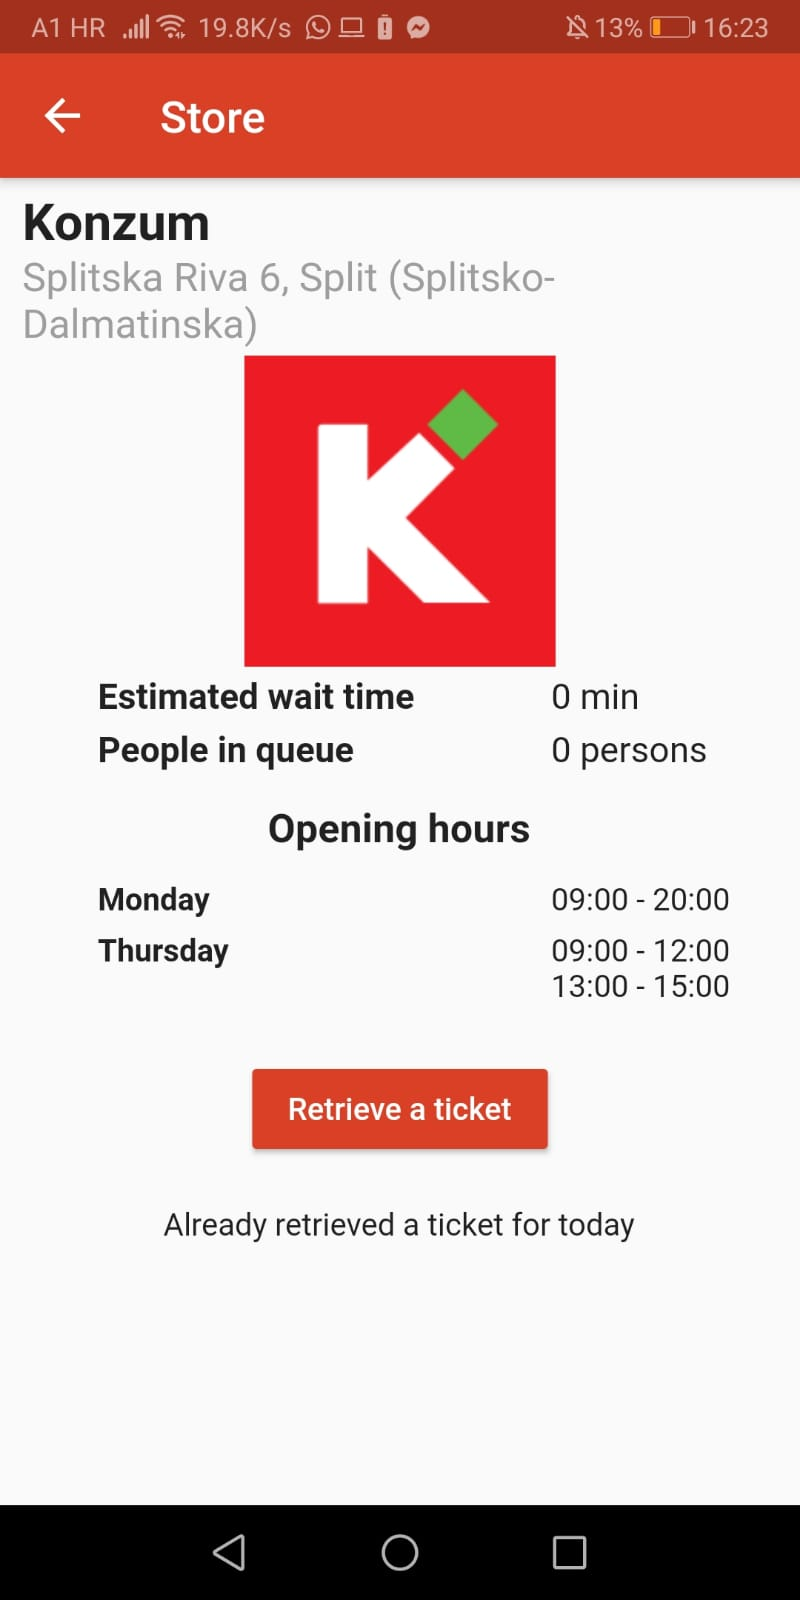
\includegraphics[width=0.9\textwidth]{Images/AlreadyRetrieved}
\captionsetup{justification=centering}
\caption{\label{fig:appandroiderr1}\textbf{Ticket already retrieved for the same store that day (and not deleted yet)}}
\end{minipage}
\begin{minipage}{0.45\textwidth}
\centering
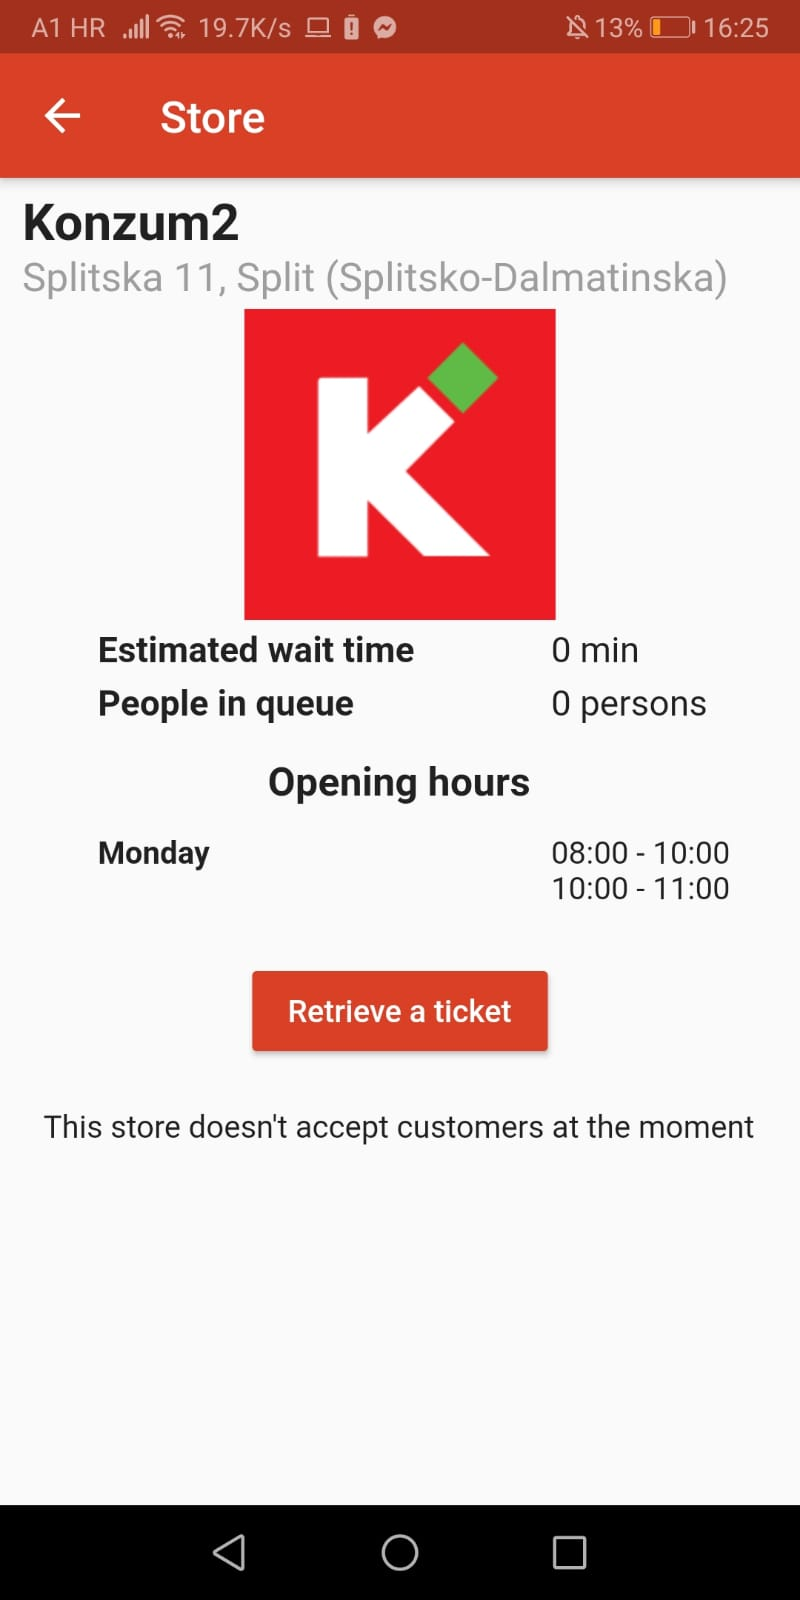
\includegraphics[width=0.9\textwidth]{Images/ClosedStore}
\captionsetup{justification=centering}
\caption{\label{fig:appandroiderr2}\textbf{The store is currently closed error}}
\end{minipage}
\end{figure}




%------------------------------------------------------------------------------------------------------------------------------------------------
\clearpage
{\color{Blue}{\section{Installation Instructions}}}
\label{sect:installationinstructions}
\hspace{\parindent} Installing and testing the app is easy.
All that needs to be done is to download .apk file from "DeliveryFolder" of our GitHub page (\url{https://github.com/robertodavinci/ Software_Engineering_2_Project_Medvedec_Sikora/tree/main/DeliveryFolder}) and install it on the phone.\newline

Make sure to allow apps from untrusted source in the settings so that the app can be properly installed since this version of the app is not signed for Google Play Store. \newline

When asked for permission to use camera, "Allow" must be pressed in order for the QR code scanner to work properly. If the camera is not allowed, the app will return to the Home screen every time a scanner is opened.\newline

There is also a possibility of importing an entire project in Android Studio and running the app on an emulator.
Simply download the whole "Implementation" folder from our repository and import the project to Android Studio. The setup should be done automatically. 


%------------------------------------------------------------------------------------------------------------------------------------------------
\clearpage
\addcontentsline{toc}{section}{References}
\bibliographystyle{plain}
\bibliography{main}
%------------------------------------------------------------------------------------------------------------------------------------------------




\end{document}
